\chapter{Lomb-Scargle diagrams}\label{appendix:Lomb-Scargle}

% The ground-based EBLMs
\begin{figure}
    \centering
    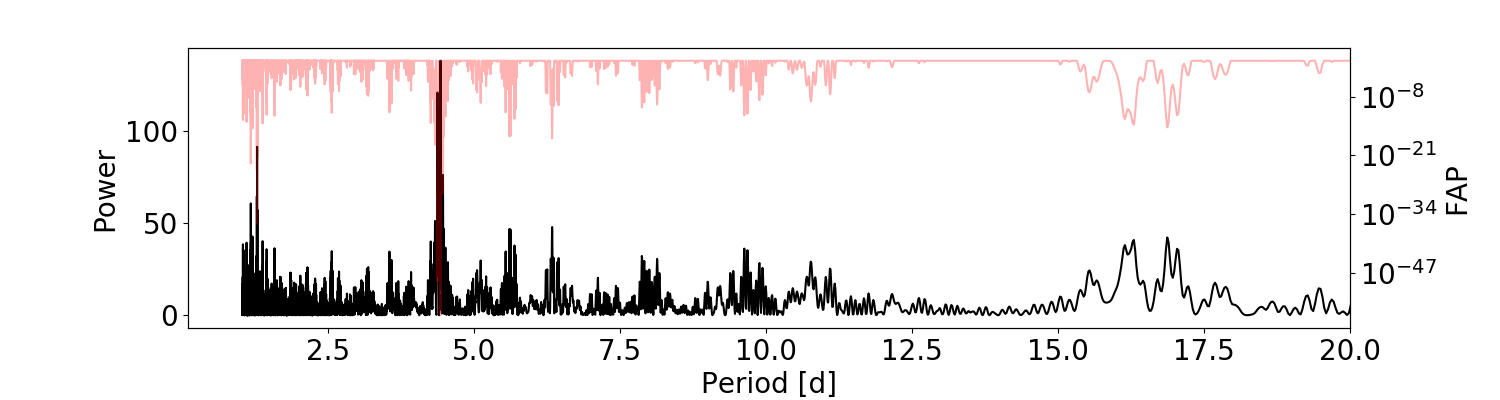
\includegraphics[scale=0.4]{Appendix/Peridograms/J2349-32_period.png}
    \caption{The generalised Lomb-Scargle diagram J2349$-$32 for WASP photometry (black) with false-alarm probabilities (FAP; red). }
    \label{appendix:fig:J2349-32_lomb}
\end{figure}

\begin{figure}
    \centering
    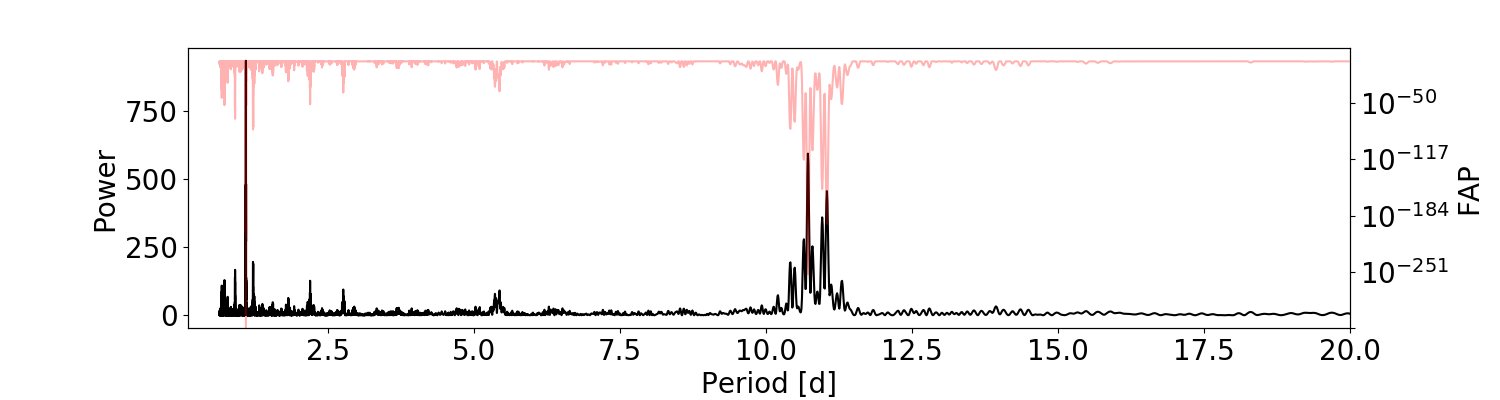
\includegraphics[scale=0.4]{Appendix/Peridograms/J2308-46_period.png}
    \caption{The generalised Lomb-Scargle diagram J2308$-$46 for WASP photometry (black) with false-alarm probabilities (FAP; red). }
    \label{appendix:fig:J2308-46_lomb}
\end{figure}

\begin{figure}
    \centering
    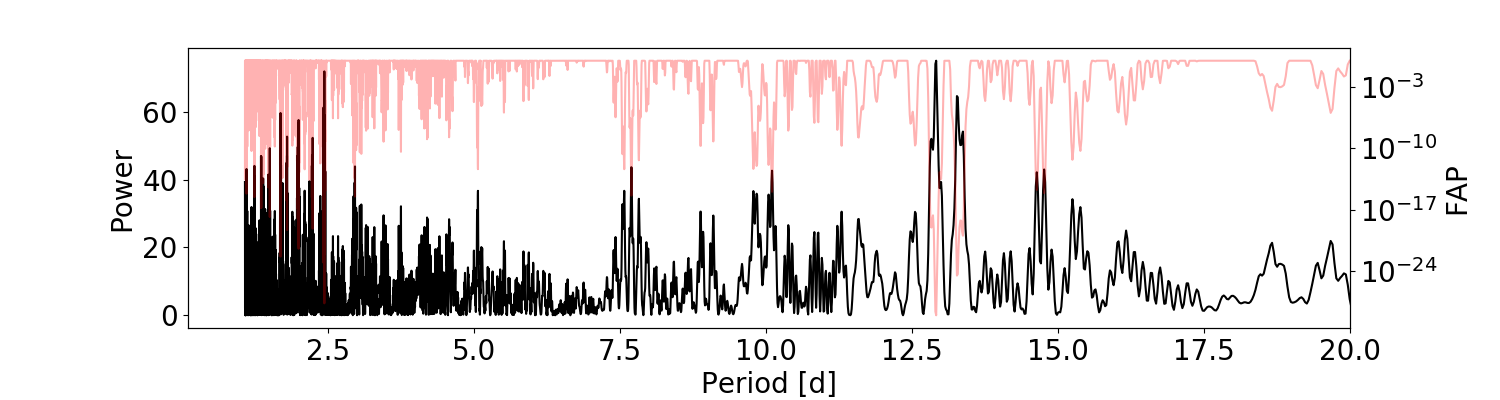
\includegraphics[scale=0.4]{Appendix/Peridograms/J0218-31_period.png}
    \caption{The generalised Lomb-Scargle diagram J0218$-$31 for WASP photometry (black) with false-alarm probabilities (FAP; red). }
    \label{appendix:fig:J0218-31_lomb}
\end{figure}

\begin{figure}
    \centering
    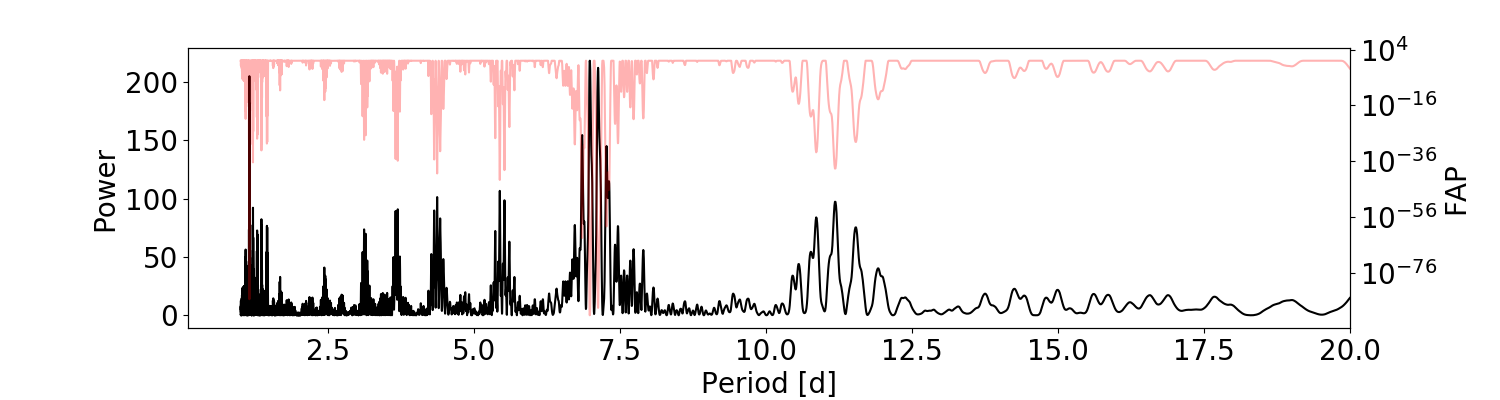
\includegraphics[scale=0.4]{Appendix/Peridograms/J1847+39_period.png}
    \caption{The generalised Lomb-Scargle diagram J1847$-$39 for WASP photometry (black) with false-alarm probabilities (FAP; red). }
    \label{appendix:fig:J1847+39_lomb}
\end{figure}

\begin{figure}
    \centering
    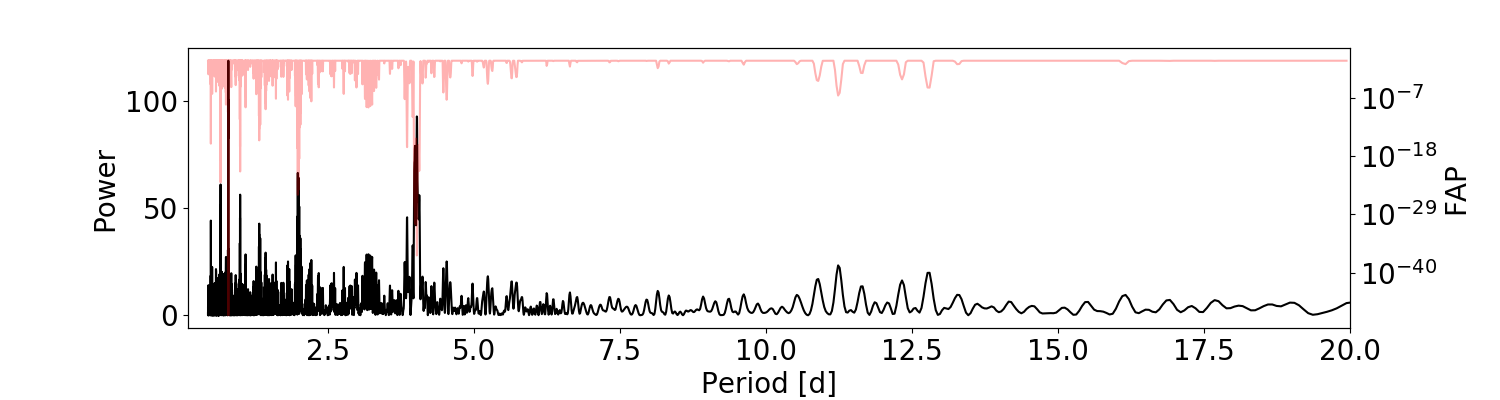
\includegraphics[scale=0.4]{Appendix/Peridograms/J1436-13_period.png}
    \caption{The generalised Lomb-Scargle diagram J1436$-$13 for WASP photometry (black) with false-alarm probabilities (FAP; red). }
    \label{appendix:fig:J1436-13_lomb}
\end{figure}

% The K2 EBLMs
\begin{figure}
    \centering
    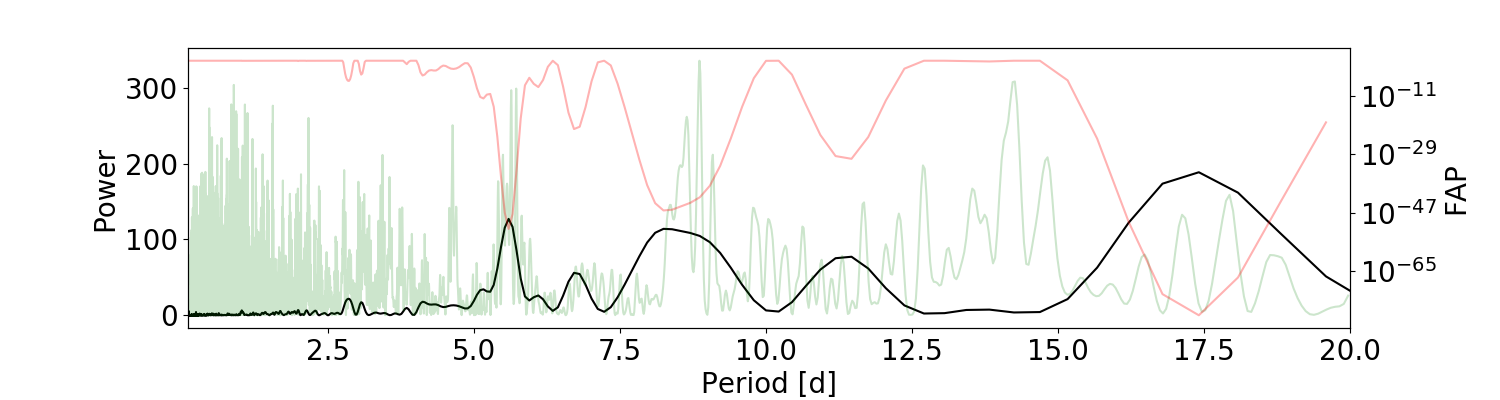
\includegraphics[scale=0.4]{Appendix/Peridograms/J0055-00_period.png}
    \caption{The generalised Lomb-Scargle diagram J0055$-$00 for K2 photometry (black) with false-alarm probabilities (FAP; red). The Lomb-Scargle diagram of WASP photometry is also shown (green).  }
    \label{appendix:fig:J0055-00_lomb}
\end{figure}

\begin{figure}
    \centering
    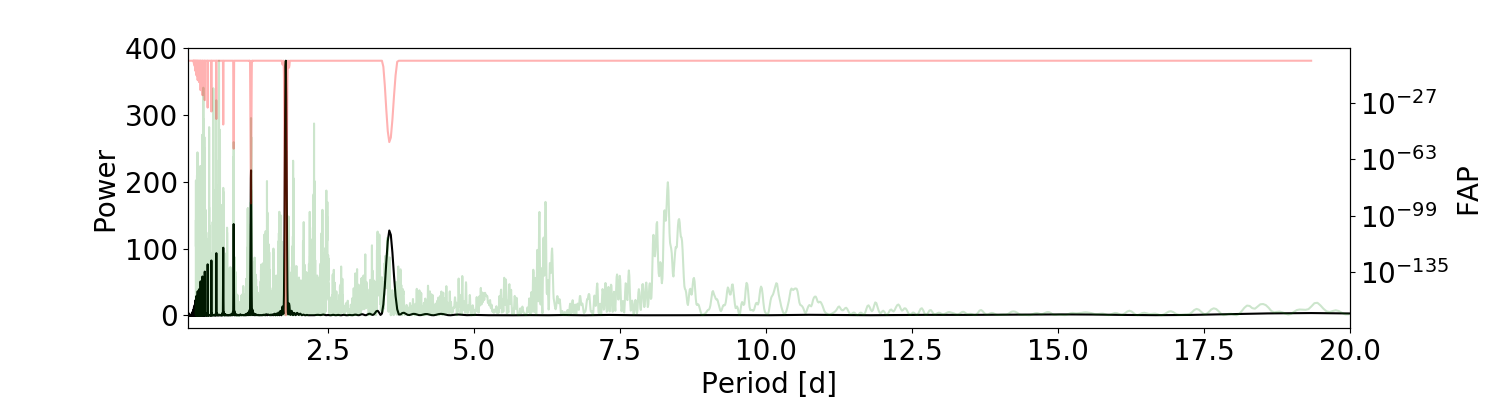
\includegraphics[scale=0.4]{Appendix/Peridograms/J0457+14_period.png}
    \caption{The generalised Lomb-Scargle diagram J0457$+$14 for K2 photometry (black) with false-alarm probabilities (FAP; red). The Lomb-Scargle diagram of WASP photometry is also shown (green).  }
    \label{appendix:fig:J0457+14_lomb}
\end{figure}

\begin{figure}
    \centering
    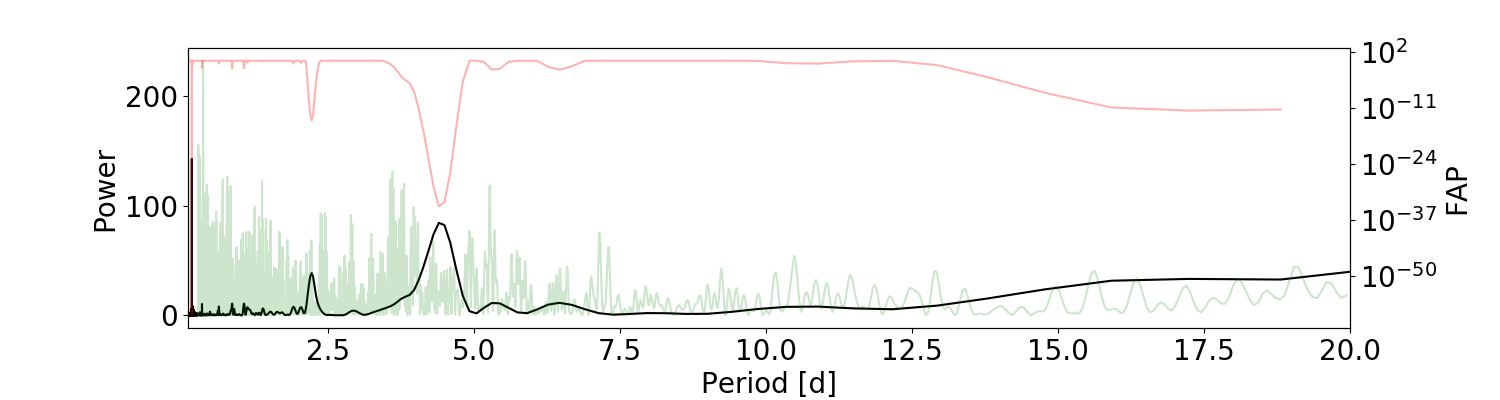
\includegraphics[scale=0.4]{Appendix/Peridograms/J1652-19_period.png}
    \caption{The generalised Lomb-Scargle diagram J1652$-$19 for K2 photometry (black) with false-alarm probabilities (FAP; red). The Lomb-Scargle diagram of WASP photometry is also shown (green).  }
    \label{appendix:fig:J1652-19_lomb}
\end{figure}